\documentclass[titlepage = firstcover]{scrartcl}
\usepackage[aux]{rerunfilecheck}
\usepackage{fontspec}
\usepackage[main=ngerman, english, french]{babel}

% mehr Pakete hier
\usepackage{expl3}
\usepackage{xparse}

%Mathematik------------------------------------------------------
\usepackage{amsmath}   % unverzichtbare Mathe-Befehle
\usepackage{amssymb}   % viele Mathe-Symbole
\usepackage{mathtools} % Erweiterungen für amsmath
\usepackage[
  math-style=ISO,    % \
  bold-style=ISO,    % |
  sans-style=italic, % | ISO-Standard folgen
  nabla=upright,     % |
  partial=upright,   % /
]{unicode-math}% "Does exactly what it says on the tin."
\usepackage[section, below]{placeins}

% Laden von OTF-Mathefonts
% Ermöglich Unicode Eingabe von Zeichen: α statt \alpha

\setmathfont{Latin Modern Math}
%\setmathfont{Tex Gyre Pagella Math} % alternativ zu Latin Modern Math
\setmathfont{XITS Math}[range={scr, bfscr}]
\setmathfont{XITS Math}[range={cal, bfcal}, StylisticSet=1]

\AtBeginDocument{ % wird bei \begin{document}
  % werden sonst wieder von unicode-math überschrieben
  \RenewDocumentCommand \Re {} {\operatorname{Re}}
  \RenewDocumentCommand \Im {} {\operatorname{Im}}
}
\usepackage{mleftright}
\setlength{\delimitershortfall}{-1sp}

%Sprache----------------------------------------------------------
\usepackage{microtype}
\usepackage{xfrac}
\usepackage[autostyle]{csquotes}    % babel
\usepackage[unicode, pdfusetitle]{hyperref}
\usepackage{bookmark}
\usepackage[shortcuts]{extdash}
%Einstellungen hier, z.B. Fonts
\usepackage{booktabs} % Tabellen


\title{Geiger-Müller-Zählrohr}
\author{
  Lasse Sternemann\\
  \href{mailto:lasse.sternemann@udo.edu}{lasse.sternemann@udo.edu}
}
\date{Bearbeitet am 23.05.2020}

\begin{document}
    \maketitle
    \newpage
    \tableofcontents
    \newpage

    \section{Theoretische Grundlagen des Geiger-Müller-Zählrohrs}
        \subsection{Aufbau}
            Das Geiger-Müller-Zählrohr besteht zunächst aus einer zylindrischen Kammer, die mit einem Gasgemisch gefüllt ist. In der Mitte diesr Kammer befindet sich ein Draht, der als Anode fungiert.
            Die innere Wand der Kammer bildet die zugehörige Kathode. Zwischen der Kathode und der Anode liegt eine Spannung von 200 bis 3000 V an, sodass ein elektrisches Feld entsteht, das aufgrund 
            der zylindrischen Form der Kammer radialsymmetrisch zur Ausrichtung des Drahts verläuft. Während der eine Deckel der Kammer abgeschlossen ist, ist auf der Seite, die bei der Nutzung auf die Quelle gereichtet ist, ein
            Mylarfenster eingebaut, das die ionisierende Strahlung in die Kammer einfallen lässt, da dieses Material eine sehr geringe Massendichte besitzt.

            \FloatBarrier

            \begin{figure}[h]
              \centering
              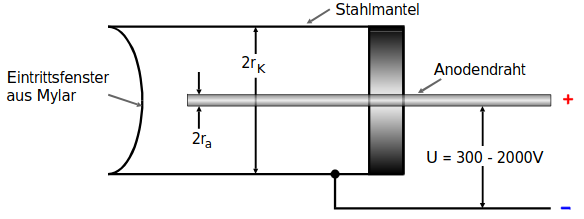
\includegraphics[width = 0.6\textwidth]{Bilder/Aufbau.png}
              \caption{In der Abbildung ist der Aufbau eines Geiger-Müller-Zählrohrs schematisch skizziert.[1]}
              \label{fig:Aufbau}
            \end{figure}

            \FloatBarrier

        \noindent
        \subsection{Funktionsbereiche des Zählrohrs}
            Da die Wechselwirkung von Photonen mit Materie mit ca. 1\% sehr gering ist die Nutzung eines Geiger-Müller-Zählrohrs nur bei hohen Intensitäten sinnvoll. Die massebehafteten $\alpha-$ und
            $\beta-$Teilchen wechselwirken jedoch beinahe zu 100\% mit den Gasatomen. Hier ist die Messung bei allen Intesitäten möglich. Daher wird diskutiert, was passiert, wenn ein geladenes
            Teilchen in die Kammer einfällt.
            Solch ein geladenes in die Kammer einfallendes Teilchen ionisiert Atome des entahltenden Gasgemisches, bis die Energie des einfallenden Teilchens nicht mehr zur Ionisation eines weiteren
            Atoms genügt. Die dabei frei werdenden Elektronen werden durch das radialsymmetrische Feld zur Anode hinbeschleunigt und dort als elektroneischer Impuls gemessen. Pro Ionisation 
            wird bei Argon eine Energie von 26 eV benötigt. So lässt über die entstandenen Impulse die Energie des einfallenden Teilchens berechnen, da diese proportional zu der Anzahl der
            Ionisationen ist. Die Anzahl der letztendlich gemessenen Impulse hängt jedoch stark von der angelegten Spannung ab, die sich in 5 Bereiche unterteilen lässt.

            \newpage
            \subsubsection*{Bereich I}
                Bei einer geringen angelegten Spannung von bis zu 50 V ist das elektrische Feld in der Kammer so gering, dass die durch Ionisation freigesetzten Elektronen zumeist Rekombinieren, bevor
                sie die Anode erreichen. So lässt sich die Intensität oder Energie der einfallenden Teilchen nicht messen.

            \subsubsection*{Bereich II}
                Wenn die angelegte Spannung zwischen 50 und 230 Volt liegt, ist das Feld stark genug, um die Rekombination von freigesetzten Elektronen beinahe komplett zu verhindern. Daher erreichen
                fast alle freigesetzten Elektronen die Anode und es kann ein Strom gemessen werden, der proportional zur Energie des einfallenden Teilchens ist. Dieser Spannungsbereich wird in
                Ionisationskammern verwendet, die zwar nur bei hohen Intensitäten funktionieren, aber dafür eine Bestimmung der Teilchenenergie erlauben. Die hohen Intensitäten sind nötig, da der 
                entstehende Strom sonst zu gering zur Messung wäre.

            \subsubsection*{Bereich III}
                Der nächsthöhere Bereich von 230 bis 770 Volt zeichnet sich dadurch aus, dass das elektrische Feld die freigesetzten Elektronen so stark beschleunigt, dass diese wieder genug Energie
                besitzen, um weiter Atome zu ionisieren. Diese Stoßionisation vervielfacht die Anzahl der Elektronen immens, sodass am Ende von einer Townsend-Lawine an Elektronen gesprochen wird. 
                Die hohe Anzahl an zur Anode wandernden Elektronen ermöglicht nun die Messung eines Ladungsimpulses pro einfallendem Teilchen. Wie in Abbildung \ref{fig:Bereiche} zu sehen ist, steigt die Anzahl der
                Ionisationen mit der Spannung, da stärker beschleunigte Elektronen mehr weiter Ionisationen bewerkstelligen. Trotz der Vervielfältigung der Elektronen ist die Anzahl der 
                Ausgangselektronen und somit auch die Gesamanzahl der Elektronen proportional zur Energie des einfallenden Teilchens und diese kann weiterhin bestimmt werden. Die immernoch vorhandene
                Proportionalität gibt Geräten, die diesen Spannungsbereich verwenden den Namen Proportionalitätszählrohr.
                
            \subsubsection*{Bereich IV}
                Der darauf folgende Bereich von 770 bis 970 Volt wird als Auslösebereich beschrieben und ist der von Geiger-Müller-Zählrohren verwendete Bereich. Die Proportionalität zwischen 
                Ionisationen und Energie des einfallenden Teilchens ist nicht mehr gegeben. Dies liegt daran, dass die freigesetzten Elektronen nun vielfach die Atome anregen, sodass diese 
                ultra-violette Photonen abgeben. Deren Energie genügt, um weiter Atome zu ionisieren. Da sie jedoch ungeladen sind, ionisieren sie Atome in allen Bereichen der Kammer, sodass nicht
                mehr eine Townsend-Lawine, sondern eine Vielzahl dieser in der gesamten Kammer entstehen. Also'hängt die Anzahl der Ionisationen von der Größe der Kammer und nicht der Energie des 
                einfallenden Teilchens ab. Das Wegfallen der Proportionalität zwischen Energie des einfallenden Teiclhens und Ionisationen verhindert die Energiebestimmung des einfallenden Teilchens.
                Die Intensität kann weiterhin gemessen werden.

            \subsubsection*{Bereich V}
                Im sogenannteb Entladungsbereich ist die angelegte Spannung so groß, dass bereits durch ein geladendes Teilchen eine fortlaufende Ionisation hervorgerufen werden kann, die zur 
                Dauerentladung führt. Dabei fallen so viele Elektronen auf die Anode, dass die hohe Stromstärke das Messgerät zerstören kann.

                \FloatBarrier

                \begin{figure}[h]
                  \centering
                  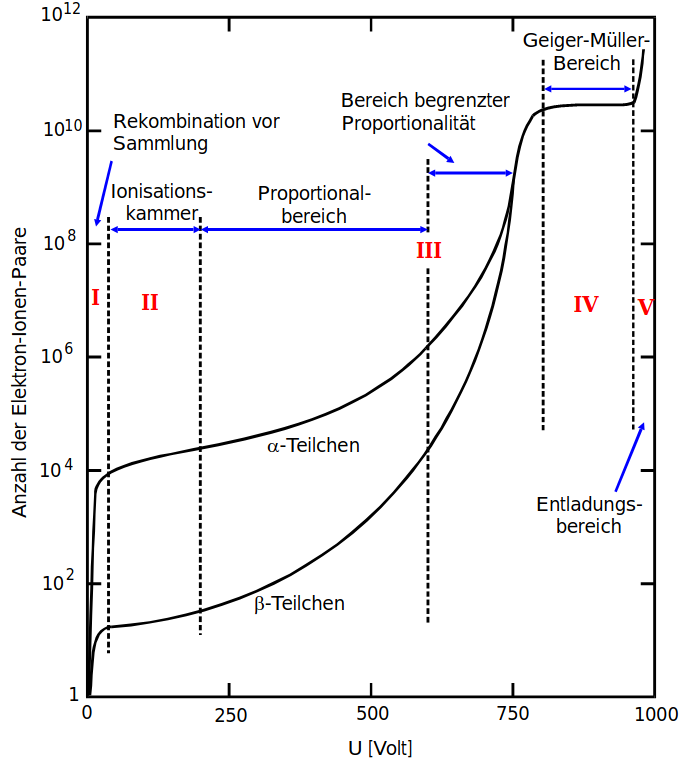
\includegraphics[width = 0.6\textwidth]{Bilder/Bereiche.png}
                  \caption{In der Abbildung sind die 5 Spannungsbereiche einer Zählkammer dargestellt. Dazu wird die Anzahl der Elektron-Ion-Paare, die der Anzahl der Ionisationen entspricht, gegen die zwischen Kathode und Anode anliegende Spannung aufgetragen. [1]}
                  \label{fig:Bereiche}
                \end{figure}
    
                \FloatBarrier
                
                \noindent
        \subsection{Totzeit, Erholungszeit und Nachentladungen}
            \subsubsection*{Totzeit}
                Sobald ein Atom ionisiert worden ist, wandert das Elektron zum Anodendraht und das ionisierte Atom zum Kathodenmantel. Während das Elektron sehr schnell die Anode erreicht, benötigt 
                das Ion aufgrund seiner höheren Masse weitaus länger. Bis das Ion den Kathodenmantel erreicht hat, besitzt es ein positives elektrisches Feld. Diese elektrische Feld wirkt dem des 
                Anodendrahts entgegen, sodass die freigesetzten Elektronen nicht die zur Stoßionisation nötige Beschleunigung erfahren und so auf dem Anodendraht keine Ladungsimpulse gemessen werden 
                können. Daher ist in der Zeitspanne, in der sich die Ionen noch nah am Anodendraht befinden, keine Messung eines einfallenden Teilchens möglich. Diese Zeitspanne wird als
                Totzeit T betitelt und ist in Abbildung \ref{fig:Zeit} zu erkennen. Aufgund dieser Totzeit ist die gemessene Intensität immer etwas geringer als die eigentlich Einfallende, da das
                Zählrohr zu Beginn nicht alle einfallenden Teilchen regestriert. Die tatsächlich einfallende Intensität $N_{\text{w}}$ berechnet sich über folgende Formel, die die gemessene Intensität 
                $N_{\text{r}}$ und einen Anteil der Integrationszeit $TN_{\text{r}}$, in der das Zählrohr einfallende Teilchen nicht regestriert.
                
                \begin{equation*}
                    N_{\text{w}} = \frac{N_{\text{r}}}{1-TN_{\text{r}}}
                \end{equation*}
                \noindent
                Wenn nun die Impulsraten von zwei verscheidenen Quellen $N_1, N_2$ und deren gemeinsamme Impulsrate $N_{1+2}$ gemessen wird, kann über die drei Formeln der wahren Impulsraten
                $N_{\text{w}_{1}}, N_{\text{w}_{2}}$ und $N_{\text{w}_{1+2}}$ und der Annahme $T^2N^2 >> 1$ eine Gleichung für die Totzeit gebildet werden.

                \begin{equation}
                    T \approx \frac{N_1 + N_2 - N_{1+2}}{2 \cdot N_1N_2}
                    \label{eqn:Totzeit}
                \end{equation}

                \noindent
            \subsubsection*{Erholungszeit}
                Während die Ionen nach außen zum Kathodenmantel wandern, sinkt der Einfluss ihres Feldes auf das der Anode mit steigendem Abstand zum Anodendraht. Daher werden die Elektronen wieder
                stark genug beschleunigt, um zumindest in geringerem Umfang Stoßionisationen durchzuführen. Da die Beschleunigung jedoch noch immer nicht der Beschleunigung des unbeeinflussten
                elektrischen Feldes der Anode entspricht, wird auf dem Anodendraht eine geringere Ladungsmemge gemessen. Die gemessene Ladungsmemge steigt an, bis die Ionen den Kathodenmantel 
                erreichen und die freigesetzten Elektronen wieder die Beschleunigung des uneingeschränkten E-Feldes der Anode erfahren. Die Zeitdauer bis zu diesem Moment wird als Erholungszeit
                beschrieben und ist ebenfalls in Abbildung \ref{fig:Zeit} zu sehen.

            \subsubsection*{Nachentladungen}
                Die notwendige Neutralisation der Ionen am Kathodenmantel geht mit der Freisetzung eines Elektrons aus dem Kathodenmantel aufgrund von überschüssiger Energie  bei der Neutralisation
                einher. Dieses freigesetzte Elektron wandert nach verstreichen von Tot- und Erholungszeit zum Anodendraht und erzeugt so den Anschein eines einfallenden Teilchens. Da dies die Messung 
                der Intensität verfäschen würde, muss dieser Prozess verhindet werden. Dazu wird dem Gas ein Alkohol hinzugegeben, auf dessen Moleküle die Ionen treffen und sie ionisieren, während sie 
                sich an ihnen entladen. Nun wandern statt der Gasionen die ionisierten Alkoholmoleküle zum Kathodenmantel. Wenn sie sich an diesem Neutralisatieren wird die überschüssige Energie durch
                Schwingungen des Alkoholmoleküls aufgenommen und so die Freisetzung eines Elektrons verhindert. 

                \FloatBarrier

                \begin{figure}[h]
                  \centering
                  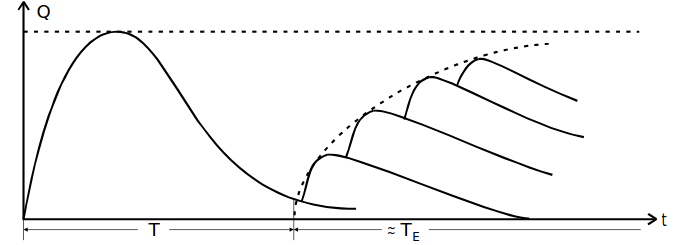
\includegraphics[width = 0.6\textwidth]{Bilder/Zeit.png}
                  \caption{In der Abbildung sind die Totzeit T und Erholungszeit $\text{T}_{\text{E}}$ schematisch dargestellt. Es ist deutlich zu erkennen, wie der Einfluss des E-Feldes der Gasionen mit der Zeit abnimmt und so die gemessene Ladungsmenge auf dem Anodendraht wieder auf das anfänglichde Niveau steigt. [1]}
                  \label{fig:Zeit}
                \end{figure}

                \FloatBarrier
            

        \subsection{Charakteristik des Geiger-Müller-Zählrohrs}
            Das Geiger-Müller-Zählrohr arbeitet in Bereich IV der Spannung. Dieser zeichnet sich durch eine konstante Intensität bei steigender Spannung aus. Dieser Bereich konstanter Intensität
            wird als Plateau bezeichnet und charakterisiert die Güte eines Geiger-Müller-Zählrohrs. Die Güte ist perfekt, wenn die Steigung des Plataeus null und das Plataeu möglichst lang ist. Da 
            trotz des hinzugefügten Alkohols noch immer geringfügig Nachentladungen auftreten, die zur Intensität hinzugezählt werden, ist das Plataeu in der Praxis nicht konstant, sondern weißt eine 
            leichte Steigung auf. Während das Plataeu dem Arbeitsbereich des Geiger-Müller-Zählrohrs entspricht, muss der sich anschließende Bereich strikt gemieden werden, da sonst wie bereits 
            beschrieben hohe Ströme das Zählrohr beschädigen.

            \FloatBarrier

            \begin{figure}[h]
              \centering
              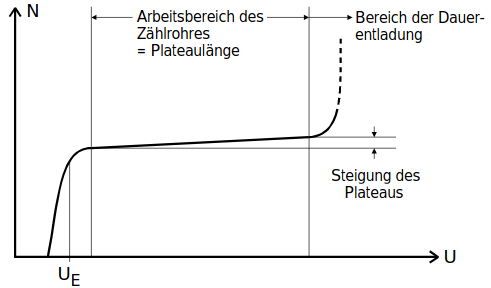
\includegraphics[width = 0.6\textwidth]{Bilder/SchemaCharakteristik.png}
              \caption{In der Abbildung ist Spannungsbereich IV und der Beginn von Spannungsbereich V detailliert dargestellt. Das eingezeichnete Plataeu markiert den tatsächlichen Arebitsbereich eines Geiger-Müller-Zählrohrs. Der sich anschließende Bereich V stellt aufgrund hoher Stromstärken eine Gefahr für das Zählrohr dar.[1]}
              \label{fig:SchemaCharakteristik}
            \end{figure}

            \FloatBarrier

        \subsection{Anodenstrom}
            Über den an der Anode anfallenden Strom kann bei gemessener Impulsrate die Menge an freigesetzter Ladung pro einfallendem Teilchen $Z$ berechnet werden. Dazu muss der momentane Anodenstrom
            $I$ durch den zugehörigen Rate der einfallenden Teilchen $N$ geteilt werden. Um die Menge der freigesetzten Ladung in Einheiten der Elementarladungladung anzugeben, muss zudem noch 
            mit dem Kehrwert der Elementarladung $e$ multipliziert werden, sodass sich folgende Formel ergibt.

            \begin{equation}
                Z =  \frac{I}{eN}
                \label{eqn:Ladung}
            \end{equation}
    
    \newpage
    \section{Durchführung}
        \subsection{Messschaltung}
            Das hier zu untersuchende Messrohr ist mit Argon gefüllt und es wird ein Thallium-204-Präperat als Strahlungsquelle genutzt.
            Zur Untersuchung des Geiger-Müller-Zählrohrs wird folgende Schaltung genutzt:

            \FloatBarrier

                \begin{figure}[h]
                  \centering
                  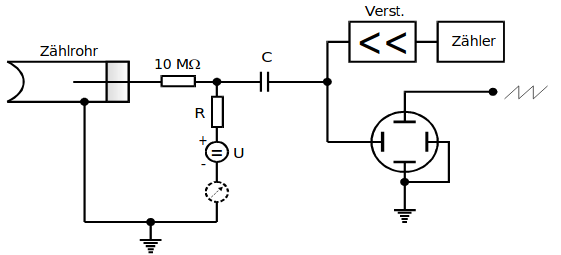
\includegraphics[width = 0.6\textwidth]{Bilder/Messaufbau.png}
                  \caption{In der Abbildung ist die Schaltung zur Untersuchung des Geiger-Müller-Zählrohrs skizziert.[1]}
                  \label{fig:Messaufbau}
                \end{figure}

            \FloatBarrier
            \noindent
            Neben der klassischen Schaltung zur Erzeugung des elektrischen Feldes ist auch die Schaltung zur Messung und Visualisierung der Ladungsimpulse zu sehen. Der über die freien Elektronen
            aufgenommene Strom fließt aus dem Anodendraht zum Widerstand und erzeugt so aus dem Ladungsimpuls einen Spannungsimpuls, der über einen Kondensator aus dem linken Stromkreis seperiert wird.
            Der seperierte Spannungsimpuls wird entweder verstärkt und gezählt oder in einem Oszilloskop graphisch dargestellt.

        \subsection{Charakteristik}
            Um die Charakteristik des verwendeten Geiger-Müller-Zählrohrs zu bestimmen wird eine konstante Intensitätsquelle in Form eines $\beta-$Strahlers vor dem Zählrohr platziert und dann unter 
            variierender Spannung im Bereich von 230 bis 700 Volt die Intensitätsrate bei einer Integrationszeit von 120 Sekunden gemessen. Es darf nicht über 700 V gegangen werden, da dann die 
            Dauerentladung einsetzt und das Gerät beschädigt wird.

        \newpage
        \subsection{Totzeit-Bestimmung}
            Die Bestimmung der Totzeit des verwendeten Geiger-Müller-Zählrohrs kann über zwei Methoden durchgeführt werden.
            
            \subsubsection*{Oszilloskop}
                Eine graphische Möglichkeit der Auswertung wird über ein Oszilloskop durchgeführt, auf dem die vom Anodendraht ankommenden Spannungsimpulse visualisiert werden. Die Totzeit 
                lässt sich über den zeitlichen Abstand zwischen dem ersten und zweiten Impuls ablesen.
                
            \subsubsection*{Zwei-Quellen-Methode}
                Eine genauere Bestimmung der Totzeit ist über die Zwei-Quellen-Methode möglich. Dazu wird zunächst eine Quelle vor den Zähler gestellt und die Intensität gemessen. Dann wird eine
                weitere Probe neben der bereits platzierten Probe platziert und die gemeinsamme Intensität gemessen. Zuletzt wird die zuerst einzeln gemessene Probe entfernt und die Intensität
                der, als zweites hinzugefügten, Probe gemessen. Aus diesen drei gemessenen Intensitäten kann die Totzeit über Formel \ref{eqn:Totzeit} berechnet werden.

                \FloatBarrier

                \begin{figure}[h]
                  \centering
                  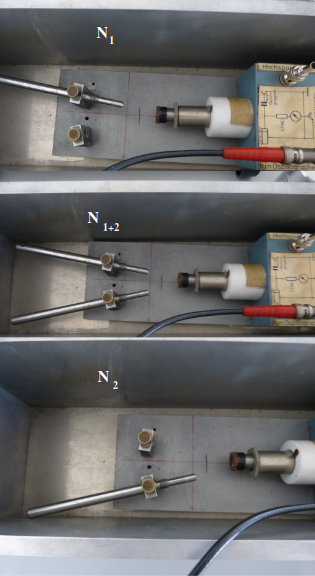
\includegraphics[width = 0.6\textwidth]{Bilder/zweischema.png}
                  \caption{In der Abbildung sind die 3 verschiedenen Aufbaue zur Messung der Totzeit über die Zwei-Quellen-Methode dargestellt. [1]}
                  \label{fig:zweischema}
                \end{figure}
            
               \FloatBarrier
               \noindent
            
        
        \subsection{Freigesetzte Ladungen}
            Um die Menge der pro einfallendem Teilchen freigesetzte Ladung zu bestimmen wird der Zählrohrstrom bei bei verschiedenen Paaren von Spannung und Intensität gemessen. Die Messungen wird 
            im Bereich von 350 bis 700 V in 50 V Schritten durchgeführt. Dabei wird eine Integrationszeit von 60 Sekunden verwendet.
            
    \newpage
    \section{Auswertung}
        \subsection{Charakteristik des Geiger-Müller-Zählrohrs}
                Zur Untersuchung der Charakteristik wird zunächst die gemessene Intensität gegen die Betriebsspannung des Geiger-Müller-Zählrohrs bei einer Integrationszeit von 60 s (Tabelle
                \ref{tab:Kennwerte}) in einer Grafik aufgetragen. Da die gemessenen Impulse $N$ poisson-verteilt sind, kann deren Fehler wie folgt berechnet werden:

                \begin{equation*}
                    \Delta N = \sqrt{N}
                \end{equation*}

                \FloatBarrier

                 \begin{figure}[h]
                   \centering
                   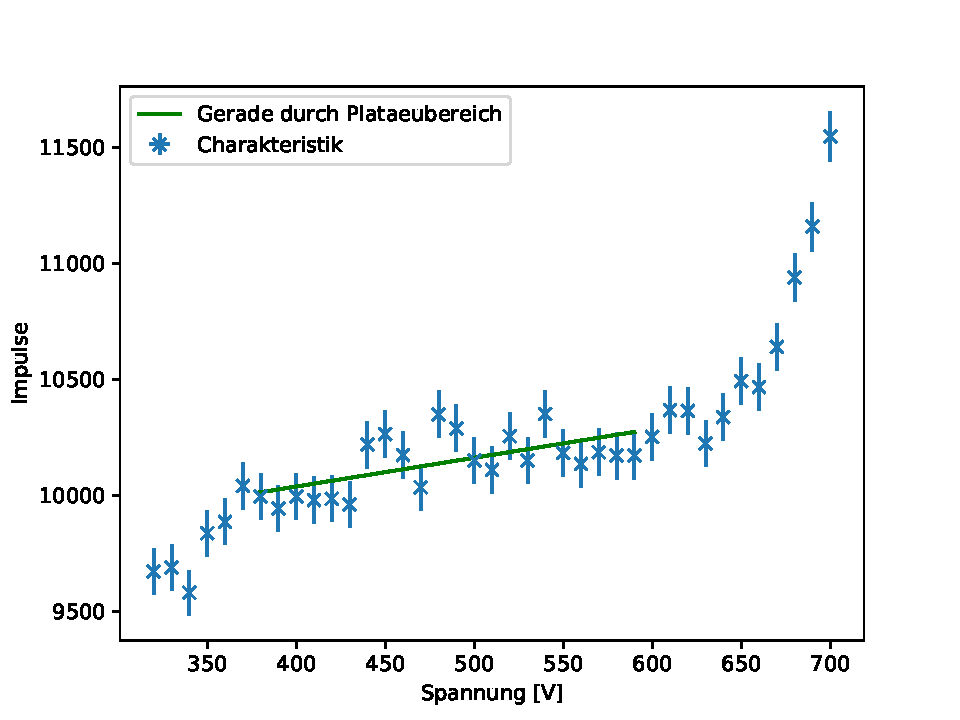
\includegraphics[width = 0.9\textwidth]{Charakteristik.pdf}
                   \caption{In der Grafik sind die gemessenen Impulse $N$ gegen die Betriebsspannung $U$ des Geiger-Müller-Zählrohrs aufgetragen. Zudem wurde eine lineare Ausgleichsgerade durch den Plataeubereich gelegt, um die Güte des Geiger-Müller-Zählrohrs zu bestimmen.}
                   \label{fig:Charakteristik}
                 \end{figure}
             
                \FloatBarrier
                \noindent
                Aus Grafik \ref{fig:Charakteristik} wird der Plataeubereich, in dem das Geiger-Müller-Zählrohr arbeitet zwischen folgenden Spannungen ermittelt:

                \begin{equation}
                    \text{Plataeubereich:}\,\, 380 \, \text{V} \. - \. 590 \, \text{V}
                \end{equation}
                \noindent
                Über diesen Plataeubereich wird eine Ausgleichsgerade zur Ermittlung der Steigung im Plataeubereich gelegt. Die lineare Regression mit der scipy-Funktion curvefit liefert
                folgende Parameter:

                \begin{align*}
                    N &= mU + b \\
                    m &= \left(1,2386 \pm 0,3774\right) \frac{1}{V} \\
                    b &= \left(9543,0095 \pm 182,5730\right)
                \end{align*}
                \noindent
                Die Güte des Geiger-Müller-Zählrohrs wird über die Steigung des Plataeubereichs $M$ angegeben. Da diese in Zunahme in \% pro 100 V angegeben wird, kann sie wie folgt über die 
                berechnete lineare Regression bestimmt werden:

                \begin{align}
                    M &= 1-\frac{\left(m \cdot 400 V + b\right)}{\left(m \cdot 500 V + b\right)} = \left(1,2 \pm 0,35\right) \, \% \, \text{pro} \, \text{100 V} \\
                    \text{mit} \, \Delta M &= \sqrt{\left(\frac{1}{\left( m \cdot 500 V + b \right)} \cdot \Delta \left(m \cdot 400 V + b\right) \right)^2 + \left( \frac{ \left(m \cdot 400 V + b \right)}{\left(m \cdot 500 V + b \right)^2} \cdot \Delta \left(m \cdot 500 V + b \right)\right)^2}
                \end{align}


        \subsection{Totzeit-Bestimmung}
            \subsubsection*{Zwei-Quellen-Methode}
                Zunächst wird die Messung für die zwei Quellen Methode durchgeführt und es ergeben sich folgende Impulsraten deren Fehler aufgrund der Poisson-Verteilung wieder über die Wurzel
                der Werte berechnet werden. 

                \begin{equation}
                    N_1 = \frac{(96941 \pm 310)}{60} \qquad N_2 = \frac{(76518 \pm 277)}{60} \qquad N_{1+2} = \frac{(158479 \pm 399)}{60}
                \end{equation}
                \noindent
                Über Formel \ref{eqn:Totzeit} wird aus den obrigen Werten die Totzeit ausgerechnet.

                \begin{equation}
                    T_2 \approx \left(115 \pm 5\right) \, \mu \text{s} \, \text{mit} \, \Delta T = \sqrt{\left(\frac{N_{1+2}-N_1}{2N_1N_2^2} \cdot \Delta N_2\right)^2 + \left(\frac{N_{1+2}-N_2}{2N_2N_1^2} \cdot \Delta N_1\right)^2 + \left(-\frac{1}{2N_1N_2} \cdot \Delta N_{1+2}\right)^2}
                \end{equation}

            \subsubsection*{Visuelle Methode}   
                Zur Bestimmung der Totzeit muss der Abstand zwischen dem Ersten Großen und ersten kleineren Peak in der visuellen Darstellung der Spannungsimpulse durch das Oszilloskop abgelesen 
                werden. Dieser zeitliche Abstand entspricht gemäß Grafik \ref{fig:Zeit} der Totzeit.  Aus Abbildung \ref{fig:Zeit} lässt sich die Totzeit $T_{\text{vis}}$ ablesen.

                \begin{equation*}
                    T_{\text{vis}} \approx 100 \mu s \qquad \text{mit} \qquad \text{1 Kästchen} \equiv 100 \mu s
                \end{equation*}

                \FloatBarrier

                \begin{figure}[h]
                  \centering
                  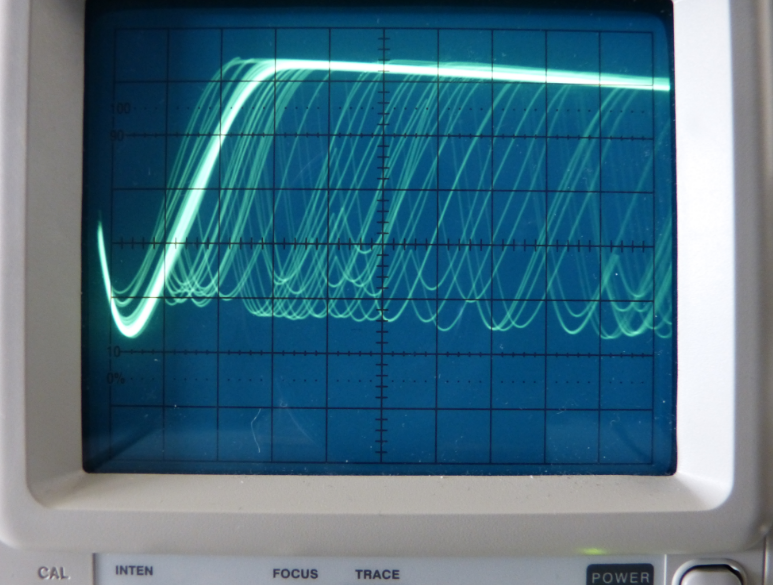
\includegraphics[width = 0.6\textwidth]{Bilder/Visuell.png}
                  \caption{In der Abbildung ist eine Aufnahme des Oszilloskopbildes zur Visualisierung der Spannungsimpulse auf dem Anodendraht. Ein Kästchen entspricht dabei einem zeitlichen Abstand von 100 $\mu s$. [1]}
                  \label{fig:Zeit}
                \end{figure}

            \FloatBarrier
            \noindent



        \subsection{Freigesetzte Ladung}
            Die Menge der freigesetzten Ladung pro einfallendem Teilchen wird über Formel \ref{eqn:Ladung} und folgendem Fehler berechnet.

            \begin{equation*}
                \Delta Z = \sqrt{\left(\frac{1}{eN} \cdot \Delta I\right)^2 + \left( \frac{-I}{eN^2} \cdot \Delta N\right)^2}
            \end{equation*}
            \noindent
            Aus den Messwerten ergeben sich folgende Werte,

            \begin{table}[h]
                \centering
                \caption{In der Tabelle sind Wertepaare aus Anodenstrom und Impulsrate, sowie die daraus berechnete freigesetzte Ladung pro einfallendem Teilchen eingetrage.}
                \label{tab:Ladungen}
                \begin{tabular}{c c c }
                    \toprule
                    {I [nA]} & {Impulsrate [1/s]} & {Z [$e \cdot 10^{10}$]} \\
                    \midrule
                    $300 \pm 50$ & $164 \pm 2$ & $1,14 \pm 0,19$\\
                    $400 \pm 50$ & $167 \pm 2$ & $1,50 \pm 0,19$\\
                    $700 \pm 50$ & $171 \pm 2$ & $2,55 \pm 0,18$\\
                    $800 \pm 50$ & $169 \pm 2$ & $2,95 \pm 0,19$\\
                    $1000 \pm 50$ & $170 \pm 2$ & $3,68 \pm 0,19$\\
                    $1300 \pm 50$ & $171 \pm 2$ & $4,75 \pm 0,19$\\
                    $1400 \pm 50$ & $175 \pm 2$ & $5,00 \pm 0,18$\\
                    $1800 \pm 50$ & $192 \pm 2$ & $5,84 \pm 0,17$\\
                     
                    \bottomrule
                \end{tabular}
            \end{table}
            \noindent
            die zudem in einem ZI-Diagramm aufgetragen werden.

            \FloatBarrier

                 \begin{figure}[h]
                   \centering
                   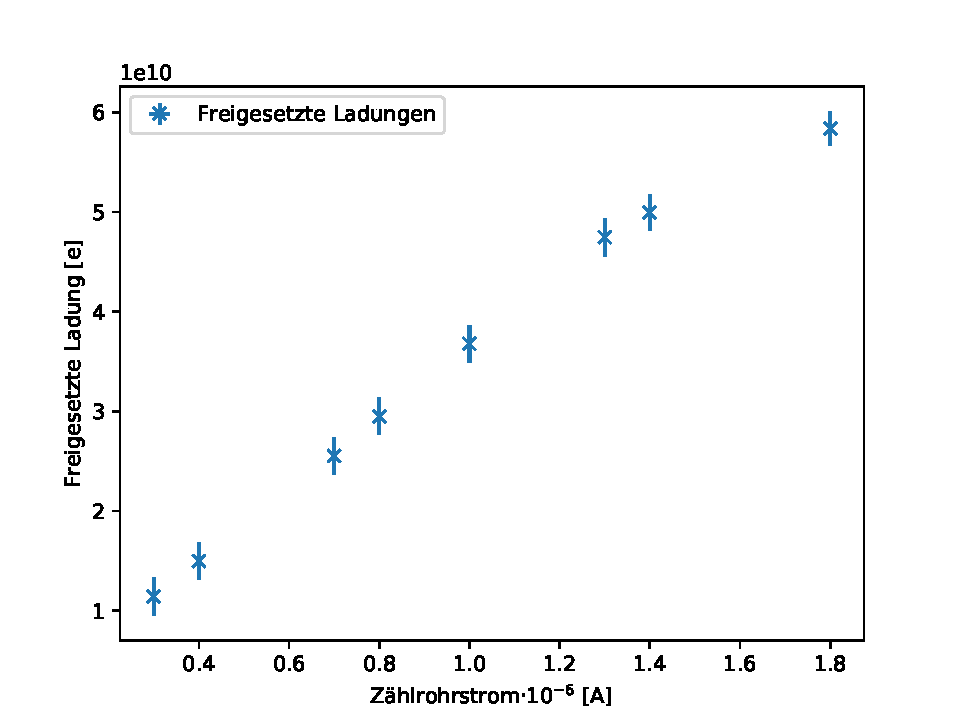
\includegraphics[width = 0.9\textwidth]{Ladungen.pdf}
                   \caption{In der Grafik sind die berechneten freigesetzten Ladungen in Einheiten der Elementarladung $e$ gegen die zugehörigen Stromstärken des Anodenstroms aufgetragen.}
                   \label{fig:Ladungen}
                 \end{figure}
             
            \FloatBarrier

            \noindent
            Diese Grafik gibt einen linearen Zusammenhang zwischen freigesetzten Ladungen pro einfallendem Teilchen und dem Anodenstrom wieder.

        \newpage
        \subsection{Diskussion}
            Die Untersuchung der charakteristik des Geiger-Müller-Zählrohrs konnte folgende Eigenschaften des Zählrohrs ermitteln.
            \begin{align*}
                \text{Plataeubereich:}&\,\, 380 \, \text{V} \. - \. 590 \, \text{V} \\
                \text{Plataeusteigung/100 V:}&\, \left(1,2 \pm 0,35\right) \, \% 
            \end{align*}
            \noindent
            Zudem ist aus Grafik \ref{fig:Charakteristik} zu erkennen, dass Betriebsspannung über 650 V vermieden werden müssen, da hier der Bereich der Selbstentladung einsetzt und Betrieb unter 
            dieser Spannung das Zählrohr beschädigen würde. \newline
            Die Werte der beiden Totzeiten
            \begin{equation*}
                T_{\text{vis}} \approx 100 \mu s \qquad T_2 \approx \left(115 \pm 5\right) \, \mu \text{s}
            \end{equation*}
            \noindent
            weichen um nicht mehr als 15 \% voneinander ab und liegen beide in der für Geiger-Müller-Zählrohre typischen Größenordnung von 100 $\mu s$.
            Die zuletzt berechneten freigesetzte Ladung pro einfallendem Teilchen \ref{tab:Ladungen} sollte proportional zur auf der Anode gemessenen Stromstärke sein. Dies lässt sich über 
            Grafik \ref{fig:Ladungen} bestätigen.  
            \newline
            Insgesamt hat die Untersuchung des Zählrohrs die typischen Eigenschaften und Parameter eines Geiger-Müller-Zählrohrs bestätigt.
                 

        
        \newpage
        \section{Literaturverzeichnis}
                [1] \textit{Versuchsanleitung V703 - Das Geiger-Müller-Zählrohr.} TU Dortmund, 2020 
              
            
            \newpage
            \begin{table}[h]
                \centering
                \caption{In der Tabelle sind Wertepaare aus Betriebsspannung des Zählrohrs U und gemessenen Impulsen bei einer Integrationszeit von 120 Sekunden eingetragen.}
                \label{tab:Kennwerte}
                \begin{tabular}{c c c }
                    \toprule
                    {U [V]} & {Impulse} \\
                    \midrule
                    320 &	$9672   \pm 99 $ \\
                    330 &	$9689   \pm 99 $ \\
                    340 &	$9580   \pm 98 $ \\
                    350 &	$9837   \pm 100$ \\
                    360 &	$9886   \pm 100$ \\
                    370 &	$10041  \pm 101$ \\
                    380 &	$9996   \pm 100$ \\
                    390 &	$9943   \pm 100$ \\
                    400 &	$9995   \pm 100$ \\
                    410 &	$9980   \pm 100$ \\
                    420 &	$9986   \pm 100$ \\
                    430 &	$9960   \pm 100$ \\
                    440 &	$10219  \pm 102$ \\
                    450 &	$10264  \pm 102$ \\
                    460 &	$10174  \pm 101$ \\
                    470 &	$10035  \pm 101$ \\
                    480 &	$10350  \pm 102$ \\
                    490 &	$10290  \pm 102$ \\
                    500 &	$10151  \pm 101$ \\
                    510 &	$10110  \pm 101$ \\
                    520 &	$10255  \pm 102$ \\
                    530 &	$10151  \pm 101$ \\
                    540 &	$10351  \pm 102$ \\
                    550 &	$10184  \pm 101$ \\
                    560 &	$10137  \pm 101$ \\
                    570 &	$10186  \pm 101$ \\
                    580 &	$10171  \pm 101$ \\
                    590 &	$10171  \pm 101$ \\
                    600 &	$10253  \pm 102$ \\
                    610 &	$10368  \pm 102$ \\
                    620 &	$10365  \pm 102$ \\
                    630 &	$10224  \pm 102$ \\
                    640 &	$10338  \pm 102$ \\
                    650 &	$10493  \pm 103$ \\
                    660 &	$10467  \pm 103$ \\
                    670 &	$10640  \pm 104$ \\
                    680 &	$10939  \pm 105$ \\
                    690 &	$11159  \pm 106$ \\
                    700 &	$11547  \pm 108$ \\
                    \bottomrule
                \end{tabular}
            \end{table}
        \noindent
            
        \end{document}